\subsection{Calorimeters}

The calorimeters are designed to measure the energy from particles by absorbing them.
They are located outside the solenoidal magnet that surrounds the inner detector.
The ATLAS calorimeters are comprised of a series of full $\phi$-symmetrical sampling calorimeters with the pseudorapidity range of $|\eta|<4.9$.
Figure~\ref{fig:calo_dec} shows the layout of the ATLAS calorimeter system.
There are two basic calorimeter systems: an inner electromagnetic (EM) calorimeter and an outer hadronic calorimeter.
The EM calorimeter is designed for precise measurements of electrons and photons with fine granularity;
while the hadronic one has relative coarser granularity but satisfies the physics requirements for jets reconstructions and $E_{T}^{miss}$ measurements.
Two different sampling techniques are used, the EM calorimeter is purely based on liquid-argon (LAr) technology, while the hadronic one use both LAr and scintillating tiles calorimeters. 
More details are described as below:
\begin{figure}[!htb]
  \centering
  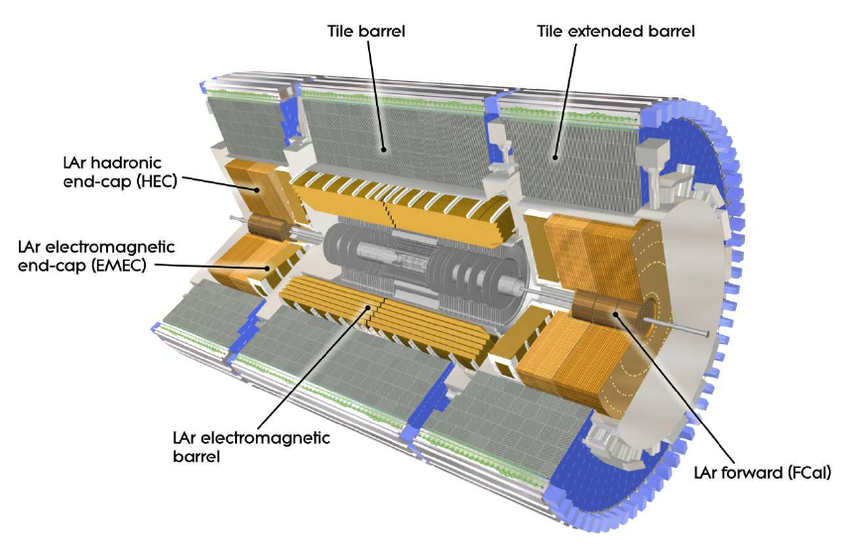
\includegraphics[width=0.8\textwidth]{figures/Detector/calo_layout.png}
  \caption{Layout of the ATLAS calorimeters. The scintillator-based tile hadronic calorimeters are seen outside the LAr calorimeters~\cite{Buchanan:2008}.}
  \label{fig:calo_dec}
\end{figure}

%% ================================ LAr calorimeter ===================
\textbf{Liquid Argon calorimeter}

The LAr calorimeter uses liquid-argon as active medium.
The LAr sampling calorimeter technique with ``accordion-shaped" electrodes is used for all electromagnetic calorimetry covering the pseudorapidity range of $|\eta|<3.2$;
and for hadronic calorimetry with range from $|\eta| = 1.4$ to the acceptance limit $|\eta| = 4.9$~\cite{CERN-LHCC-96-041}.
Figure~\ref{fig:calo_lar} depicts a segment of the barrel calorimeter, which had ``accordion-shaped" electrodes and absorber.
For barrel EM calorimeter, the absorbing material is lead-liquid argon, while the hadronic end-cap calorimeter uses copper plates.
In addition, the forward calorimeter is split into three parts, an EM sector in which copper is used as absorbing material and two hadronic sectors using tungsten outside the EM sector.
\begin{figure}[!htb]
  \centering
  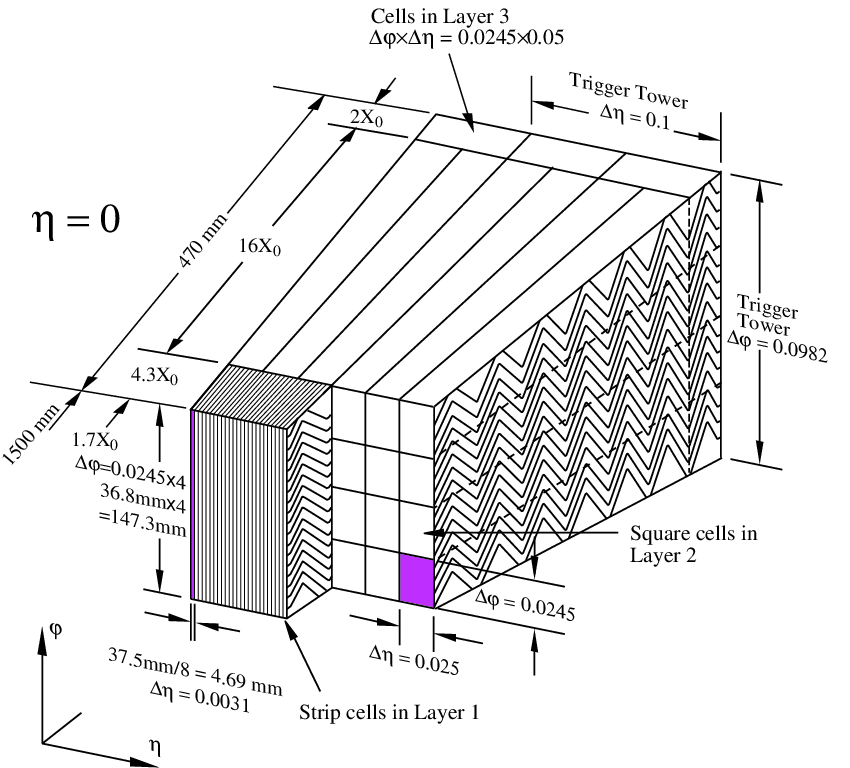
\includegraphics[width=0.6\textwidth]{figures/Detector/calo_lar.png}
  \caption{Layout of a LAr EM calorimeter barrel module~\cite{CERN-LHCC-96-041}.}
  \label{fig:calo_lar}
\end{figure}

%% =============================== Tile calorimeter ====================
\textbf{Tile calorimeter}

Tile calorimeter is a sampling calorimeter using scintillating plates as active medium and steel as absorber.
It consists of three sections: the central barrel with the pseudorapidity range of $|\eta|<1.0$ and two extended barrels with $0.8 < |\eta| < 1.7$.
Figure~\ref{fig:calo_tile} shows the design of one tile calorimeter module.
It's used for energy reconstruction of jets and $E_{T}^{miss}$ measurement by combining the measurements with the end-cap and forward LAr hadronic calorimeter.
\begin{figure}[!htb]
  \centering
  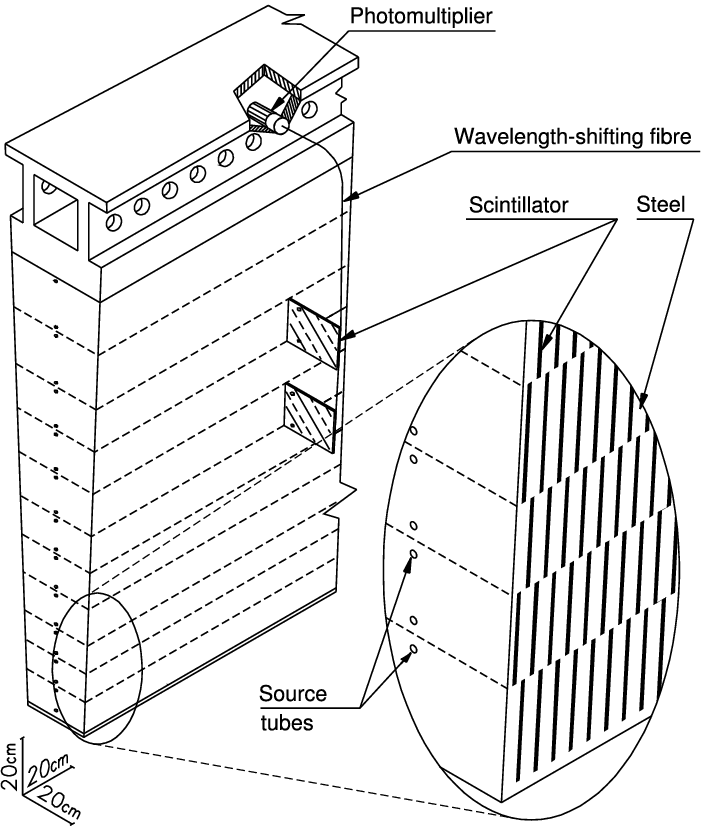
\includegraphics[width=0.5\textwidth]{figures/Detector/calo_tile.png}
  \caption{Schematic of tile calorimeter module~\cite{Aad:2010}.}
  \label{fig:calo_tile}
\end{figure}

